% Chapter 1

\chapter{Introduction} % Main chapter title

\label{Chapter1} % For referencing the chapter elsewhere, use \ref{Chapter1} 

\lhead{Chapter 1. \emph{Introduction}} % This is for the header on each page - perhaps a shortened title

%----------------------------------------------------------------------------------------

\section{Introduction to Human Robot Interaction}
	Human-Robot Interaction (HRI) is a multidisciplinary field concerned with the “analysis, design, modeling, implementation and evaluation of robots for human use”\cite{fong2003collaboration}. \textbf{\emph{HRI is a challenging research field at the intersection of psychology, cognitive science, social sciences, artificial intelligence, computer science, robotics, engineering and human-computer interaction}}\cite{dautenhahn2007methodology}. The origin of HRI as a discrete problem was stated by 20$^{\text{th}}$ century author Isaac Asimov\cite{IssacAsimov} as he stated the \emph{Three Laws of Robotics} which every HRI designer should adhere to. While this acts as one of the first works proposing the guidelines for HRI, Goodrich \cite{goodrich2007human} instead in his extensive survey proposed two main types of HRI.
\begin{itemize}
\item Remote interaction/ Tele-operation: The human and the robot are not colocated and are separated spatially or even temporally (for example, the Mars Rovers are separated from earth both in space and time). 
\item Proximate interaction: The humans and the robots are co-located (for example, service robots may be in the same room as humans).
\end{itemize}
	Proximate interaction has gained importance due to the successful encounters of putting robots to work with human beings. It has led to the development of a new class of robots called Social Robots. The extensive survey conducted by Fong et al.,\cite{fong2003survey} on social robots araised some of the most important questions that have to be addressed in developing an engaging HRI system. Fong et al. \cite{fong2003survey} define that social robots are able to recognize each other and engage in social interactions; Breazeal et al.\cite{Breazeal:2002:DSR:515422} explain that a social robot is a robot which is able to communicate with humans in a personal way; Bartneck and Forlizzi \cite{bartneck2004design} describe that a social robot is an autonomous or semi-autonomous robot that interacts with humans by following some social behaviors; Hegel et al. \cite{hegel2009understanding} define that a social robot is a combination of a robot and a social interface. Summarizing all these Yan et al. \cite{yan2014survey} defines \emph{“A social robot is a robot which can execute designated tasks and the necessary condition turning a robot into a social robot is the ability to interact with humans by adhering to certain social cues and rules.”}. 
	
	The social robots already entered the human spaces as entertainers, educators\cite{NaoTheRobot} and caring agents\cite{ASKNao}. Given that social robotics has emerged as a promising field, designing and developing interaction systems need to be approached in a systematic manner wherein the robots should be able to understand and interact with the environment (man and materials) in a better way. To make it possible it is necessary to develop robotic systems with essential cognitive skills for efficient and natural interaction. Most often the onboard sensors on the robots fail to satisfy this demanding requirement. Hence consideration of using exteroceptive sensors to this purpose is important.  
	
	The HRI designers are from diverse backgrounds. So the tools needed to design behaviors of a social robot should be intuitive and user friendly. However when it comes to designing complex behaviors, traditional flow chart based approaches\cite{Choregraphe} increase the cognitive load of the users as they have to hand tailor all the data flow and reactiveness. More efficient tools are needed which could tackle this issue. 
	
	The main contribution of this thesis will be to develop an application independent experimental platform wherein a social robot will be equipped with essential perceptual ability to understand human motions. The behavior design of such a social robot will be made possible by efficient behavioral framework. The experimental platform will be used to design and evaluate the interaction between the social robot and the human.	

\section{Problem Statement}
\label{sec:problem_statement}
	Human Robot interaction in social context has been studied rigorously due to the potential applications foreseen. For an effective interaction, the robot has to understand precisely its environment especially the human actions and deeds. The main focus of this study will be to understand the non-verbal aspect of the interaction (i.e., visual but not auditory). For visual understanding of human intention/motion the robot has to be equipped with exceptional perception system. Due to the various considerations like portability, on board processing capability and power consumption, most often the choice of on-board sensors is compromised. Eventually the precision of the sensor information from the onboard sensors are not enough for complete understanding of human motions. In such cases there is a need to use exteroceptive sensors which are practical to be used in a social scenario while at the same time powerful enough to satisfy the requirements. This problem boils down to \emph{Selection of Sensors} which are cheap, powerful and have sufficient tools for development. Moreover it requires the study on \emph{Human motion understanding} and \emph{Localization/Tracking} of humanoid robot.
	
	Secondly, the software frameworks available to design an interaction scenario are most often not scalable. This is mainly due to the trade-off between usability and capability of defining complex dynamic behaviors. There is a need to choose one among various available software frameworks, which allow us to define dynamic behaviors. This requires the study of existing \emph{Behavioral frameworks}.

	Thirdly, we have to put the perception system work under the framework of our choice and design appropriately the information flow. Finally there is also the need to evaluate the interaction by carefully designing the scenario and study the interaction metrics using data collection methods and statistical analysis. This requires the study of \emph{HRI design and evaluation techniques}.

	Considering all the above factors we could understand the need of an application independent experimental platform for studying the human-robot interaction understanding the human motions. Figure~\ref{fig:problemstatement} depicts the possible questions this thesis will try to investigate and propose solution. 

\begin{figure}[H]
\centering
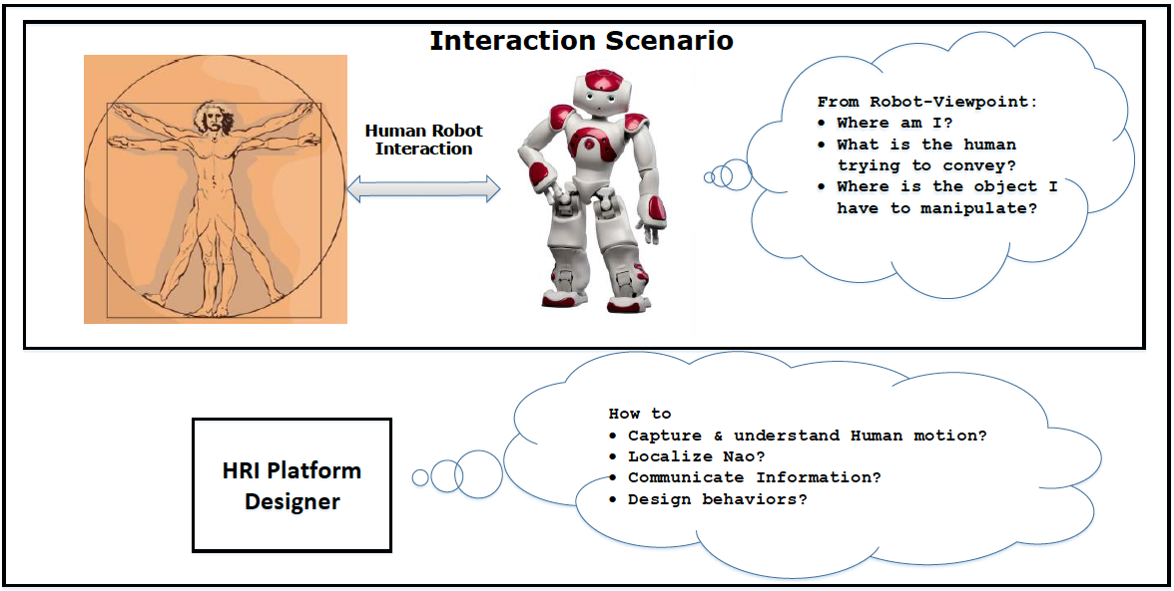
\includegraphics[width=\textwidth]{assets/ProblemStatement.png}
\caption{Concise depiction of problem statement}
\label{fig:problemstatement}
\end{figure}% 

	This bibliographic study will summarize the state-of-the-art tools and techniques available in order to address each of the problem statements described above.

\section{Organization of the report}
	The report is organized as follows. This chapter (Chapter~\ref{Chapter1}) introduced the topic of human-robot interaction and the problem statements of this thesis. Chapter~\ref{Chapter2} will give an overview of the system components like the humanoid robot and the perception system. Chapter~\ref{Chapter3} will describe the state of the art techniques on human pose estimation and gesture recognition. Chapter~\ref{Chapter4} will describe various techniques to localize and track the humanoid robot. Chapter~\ref{Chapter5} will present a study on the available robot behavioral design frameworks. Following this Chapter~\ref{Chapter6} will describe HRI design and evaluation techniques. Finally Chapter~\ref{Chapter7} presents an initial proposal of the experimental platform and provides some concluding remarks.